\chapter{\textit{Branch-and-Price}}

Neste capítulo será abordada uma possível implementação do algoritmo \textit{Branch-and-Price} (BP) para a resolução do \textit{Bin Packing Problem} (BPP). Mais precisamente, na Seção \ref{sec:definicao} será definido o BPP; na Seção \ref{sec:algoritmo}, será fornecida uma fundamentação teórica acerca de imperantes conceitos que constituem tal algoritmo; na Seção \ref{sec:implementandoGC} serão apresentadas considerações fundamentais para a implementação da Geração de Colunas, enquanto que na Seção \ref{sec:implementandoBranching} faz-se o mesmo em relação ao \textit{branching}. Por fim, na Seção \ref{sec:instancias}, comenta-se acerca do conjunto de instâncias do problema. 

\section{Definição do Problema} \label{sec:definicao}

Nesta seção será conceituado o BPP, problema para o qual será desenvolvido ao algoritmo BP. Por definição, tal problema consiste em empacotar um conjunto de itens em \textit{bins}, de modo que a capacidade dos mesmos seja respeita e que todos esses itens sejam empacotados. Desse modo, considere as seguintes definições:

\begin{itemize}
    \item $I = \{1, ..., n\}$: conjunto de itens;
    \item $M = \{1, ..., |I|\}$: conjunto de \textit{bins};
    \item $Q$: capacidade dos \textit{bins};
    \item $w_i$: peso do item $i$, $\forall i \in I$.
\end{itemize}

Em relação às variáveis do problema, sejam:

\begin{itemize}
    \item $x_{ij} = \begin{cases}
        1, \hspace{10 mm} \text{se o item $i \in I$ for empacotado no bin $j \in M$} \\ 
        0, \hspace{10 mm} \text{c.c.}
    \end{cases}$
    \item $y_{j} = \begin{cases}
        1, \hspace{10 mm} \text{se o bin $j \in M$ for utilizado} \\ 
        0, \hspace{10 mm} \text{c.c.}
    \end{cases}$
\end{itemize}

Uma formulação matemática para esse problema foi proposta por Kantorovitch, no seu trabalho \cite{Kantorovich1960}, a qual encontra-se descrita adiante: 

% Formulacao kantorovitch
\begin{align}
    \text{min }& \sum_{j \in M} y_j & \label{eq:BPP_fo}\\
    \text{s.a }& \sum_{j \in M} x_{ij} = 1  &\forall i \in I \label{eq:BPP_r1}\\
    & \sum_{i=1}^{n} w_i x_{ij} \leq Q y_j &\forall j \in M \label{eq:BPP_r2}\\
    & x_{ij} \in \{0,1\}        &\forall i \in I, j \in M\label{eq:BPP_r3}\\
    & y_j \in \{0,1\}           &\forall j \in M \label{eq:BPP_r4}
\end{align}

A função objetivo (\ref{eq:BPP_fo}) visa a minimização do número de \textit{bins} utilizados. Por sua vez, o conjunto de restrições (\ref{eq:BPP_r1}) determina que todos os itens deverão ser empacotados. Além disso, as restrições (\ref{eq:BPP_r2}) garantem que a capacidade dos \textit{bins} será respeitada. Por fim, as restrições (\ref{eq:BPP_r3}) e (\ref{eq:BPP_r4}) definem a natureza das variáveis do problema, sendo conhecidas como restrições de integralidade. A Figura \ref{fig:BPP_example}, extraída de \cite{Bulhoes2019}, ilustra um exemplo de solução para o BPP, considerando um conjunto de 10 itens, cujos pesos são: $w_1 = 1$, $w_2 = 2$, $w_3 = 5$, $w_4 = 3$, $w_5 = 6$, $w_6 = 2$, $w_7 = 6$, $w_8 = 1$, $w_9 = 4$ e $w_{10} = 9$. Cada um dos \textit{bins} possui capacidade Q = 10. Nesse exemplo, foram necessários 5 \textit{bins} para empacotar os 10 itens considerados, conforme indicado na ilustração. 

%\begin{figure}[htpb!]
%    \centering
%    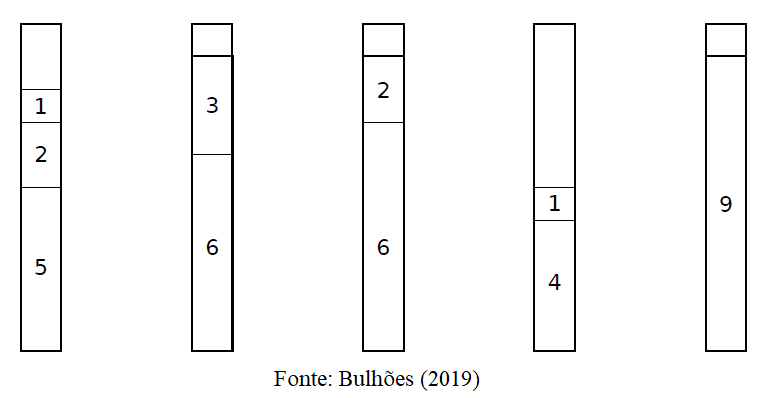
\includegraphics[scale=0.9]{imagens/ExemploBPP.png}
%    \caption{Exemplo de solução para o BPP.}
%    \label{fig:BPP_example}
%\end{figure}

% cores
\definecolor{Orange}{HTML}{ffd6a5}
\definecolor{Red}{HTML}{ffadad}
\definecolor{Yellow}{HTML}{fdffb6}
\definecolor{Blue}{HTML}{9bf6ff}
\definecolor{Green}{HTML}{caffbf}
\definecolor{Dark_blue}{HTML}{a0c4ff}
\definecolor{Violet}{HTML}{bdb2ff}

\pgfdeclarelayer{nodelayer}
\pgfsetlayers{nodelayer}

\begin{figure}[htpb!]
    \centering
    \scalebox{1.0}{
        \begin{tikzpicture}
        	\begin{pgfonlayer}{nodelayer}
        	    % bin 1
        		\node [rectangle, draw = black, minimum height = 2cm, outer sep = 0pt, minimum width = 1cm, thick] (45) at (-4, 4) {};
        		\node [rectangle, draw = black, minimum height = 1cm, outer sep = 0pt, fill=Orange, minimum width = 1cm, thick] (40) at (-4, 2.5) {$w_8$};
        		\node [rectangle, draw = black, minimum height = 2cm, outer sep = 0pt, fill=Blue, minimum width = 1cm, thick] (41) at (-4, 1) {$w_6$};
        		\node [rectangle, draw = black, minimum height = 5cm, outer sep = 0pt, fill=Red, minimum width = 1cm, thick] (42) at (-4, -2.5) {$w_3$};
        		% bin 2
        		\node [rectangle, draw = black, minimum height = 1cm, outer sep = 0pt, minimum width = 1cm, thick] (46) at (-2, 4.5) {};
        		\node [rectangle, draw = black, minimum height = 3cm, outer sep = 0pt, fill=Yellow, minimum width = 1cm, thick] (44) at (-2, 2.5) {$w_4$};
        		\node [rectangle, draw = black, minimum height = 6cm, outer sep = 0pt, fill=Green, minimum width = 1cm, thick] (43) at (-2, -2) {$w_5$};
        		% bin 3
        		\node [rectangle, draw = black, minimum height = 2cm, outer sep = 0pt, minimum width = 1cm, thick] (47) at (0, 4) {};
        		\node [rectangle, draw = black, minimum height = 2cm, outer sep = 0pt, fill=Blue, minimum width = 1cm, thick] (48) at (0, 2) {$w_2$};
        		\node [rectangle, draw = black, minimum height = 6cm, outer sep = 0pt, fill=Green, minimum width = 1cm, thick] (49) at (0, -2) {$w_7$};
        		% bin 4
        		\node[rectangle, draw = black, minimum height = 1cm, outer sep = 0pt, minimum width = 1cm, thick] (54) at (2, 4.5) {};
        		\node [rectangle, draw = black, minimum height = 9cm, outer sep = 0pt, fill=Dark_blue, minimum width = 1cm, thick] (50) at (2, -0.5) {$w_{10}$};
        		% bin 5
        		\node [rectangle, draw = black, minimum height = 5cm, outer sep = 0pt, minimum width = 1cm, thick] (53) at (4, 2.5) {};
        		\node [rectangle, draw = black, minimum height = 1cm, outer sep = 0pt, fill=Orange, minimum width = 1cm, thick] (51) at (4, -0.5) {$w_1$};
        		\node [rectangle, draw = black, minimum height = 4cm, outer sep = 0pt, fill=Violet, minimum width = 1cm, thick] (52) at (4, -3) {$w_9$};
        	\end{pgfonlayer}
        \end{tikzpicture}
    }
    \caption{Exemplo de solução para o BPP.}
    \label{fig:BPP_example}
\end{figure}


\section{Fundamentação teórica do algoritmo} \label{sec:algoritmo}
    \subsection{Simplex Revisado}
        O Simplex Revisado pode ser entendido como uma versão menos computacionalmente custosa do tradicional algoritmo Simplex desenvolvido por George Dantzig(REF). Utilizando-se de métodos eficientes na resolução de sistemas lineares e na atualização da matriz Básica inversa, é possível reduzir a complexidade de $O(m^{3} + mn)$ para $O(m^{2} + mn)$, sendo $m$ e $n$ os números de restrições e de variáveis, respectivamente. Um breve resumo do algoritmo pode ser encontrada a seguir (ref da Tabela do SR):
        % Utilizando-se apenas operações de multiplicação entre matriz e vetor na resolução de sistemas lineares e obtendo um método eficiente para atualizar a matriz Básica inversa
        
        %A seguir, as definições necessárias:
        
% NOTE(victor): nao sei se essa eh a melhor maneira de definir esses itens ae. tlvz seja necessário rever a necessidade dessas definicoes posteriormente 
        %\begin{itemize}
        %   \item $B$: matriz Básica;
        %    \item $\overline{B}$: matriz Básica atualizada;
        %    \item $A$: matriz de coeficientes;
        %    \item $b$: mão-direita;
        %    \item $x_B$: variáveis primais básicas;
        %    \item $\pi$: variáveis duais;
        %    \item $d$: direção;
        %    \item $t$: escalar positivo associado a $d$;
        %\end{itemize}
        
        %O algoritmo pode ser resumido da seguinte maneira:
        
        \begin{table}[htpb!]
        \centering
        \begin{tabular}{|p{0.015\textwidth}p{.85\textwidth}p{0.015\textwidth}|}
        \hline
         &         &  \\
         & \begin{description}
            \item[1a etapa/passo:] Define-se uma solução básica inicial $x_B$, uma matriz básica $B$ e calcula-se $B^{-1}$.
            
            \item[2o passo:] São calculados os custos reduzidos $\overline{c}$ das variáveis não básicas, por meio de $ \overline{c}_j = c_j - \pi A_j $, onde $ \pi = c_B B^{-1}$ , de maneira a selecionar qual irá fazer parte da base -- no caso, a variável que possuir o menor custo reduzido. A otimalidade é alcançada se nenhuma das possuir custo reduzido negativo. Essa etapa é conhecida como \textit{pricing}.
            
            \item[3o passo:] O vetor $ u $ que a determina direção de uma próxima solução básica $x_{\overline{B}}$ é dado por $ u = B^{-1} A_j $, sendo $A_j$ a coluna referente à variável selecionada no 2o passo/etapa.
            
            \item[4o passo:] Determina-se o escalar positivo $ t $ associado a $ u $ e à variável $x_{B(\ell)}$ que sairá da base.
            \end{description}
            
                $$\begin{aligned}
                    && t = \text{min}_{\{i = 1...m | u_i > 0\}}& \frac{x_{B(i)}}{u_i} &
                \end{aligned}$$
                
            \begin{description}
            \item[5o passo:] Seja $\overline{B} $ a matriz básica da próxima solução. Obtém-se uma nova solução básica $ x_{\overline{B}}$, onde $ x_{\overline{B}(\ell)} = t $ e $        x_{\overline{B}(i)} = x_{B(i)} - t u_i, \ \ i \neq \ell $.
                %$$ x_{\overline{B}(i)} = x_{B(i)} - t u_i, \ \ i \neq \ell $$
                %$$ x_{\overline{B}(\ell)} = t $$
            
            \item[6o passo:] $\overline{B}^{-1} $ é calculada de maneira eficiente. Essa etapa consiste na aplicação de um certo conjunto de operações elementares de linha à/na matriz $ B^{-1} $ de mareira que $\overline{B}^{-1} $ seja obtida após o processo. Tal conjunto é o mesmo necessário para que $ e_{\ell} $ seja obtido a partir de $ u $, sendo $ e_{\ell} $ um vetor unitário onde o $\ell$-ésimo elemento é igual a 1 e os demais iguais a 0. Retornasse ao 2o passo.
            
            \end{description} &  \\
         &    &  \\
 
        \hline
        \end{tabular}
        \caption{Descrição Simplex Revisado.}
        % citar o bertsimas ae
        \end{table}
        
        %Realizar o 6o passo requer aplicar um certo conjunto de operações elementares de linha na matriz $ B^{-1} $ de mareira que $\overline{B}^{-1} $ seja obtida após o processo. Tal conjunto é o mesmo necessário para que $ e_{\ell} $ seja obtido a partir de $ u $, sendo $ e_{\ell} $ um vetor unitário onde o $\ell$-ésimo elemento é igual a 1 e os demais iguais a 0.

            % 1) Solução básica inicial e cálculo prévio de B^-1
            % 2) Pricing
                % Calcular custos reduzidos e selecionar  variável para entrar na base
            % 3) Definir direção d
            % 4) Teste da razão mínima (definir escalar t)
            % 5) Atualizar Base e solução básica
            % 6) Calcular \overline{B^-1} de maneira eficiente
            
    %\subsection{Decomposição \textit{Dantzig-Wolfe}}
    %\subsection{Geração de Colunas}

\section{Implementando a Geração de Colunas} \label{sec:implementandoGC}

\section{Implementando a estrutura do \textit{branching}} \label{sec:implementandoBranching}

\section{Conjunto de instâncias} \label{sec:instancias}

Instâncias, e suas soluções ótimas, para o \textit{BPP} podem ser encontradas em \cite{bpplib}\footnote{Link direto: \url{http://or.dei.unibo.it/library/bpplib}} e possuem o seguinte formato:

\begin{table}[htpb!]
\centering
\begin{tabular}{|llll|}
\hline
 &         &                          &  \\
 & $ n $   &                          &  \\
 & $ Q $   &                          &  \\
 & $ w_i $ & $ \ \forall  i  \in  I $ &  \\
 &         &                          &  \\ \hline
\end{tabular}
\caption{Instância do \textit{BPP}.}
\end{table}

Devido a fácil compreensão das instâncias, a leitura pode ser realizada de maneira simples.